\documentclass{minimal}

\usepackage{bm}
\usepackage{tikz}
\usetikzlibrary{
	arrows.meta,
	decorations.pathmorphing,
	backgrounds,
	positioning,
	fit,
	petri,
	shapes.misc,
	graphs,
	quotes,
	decorations.pathreplacing,
	calc,
}

\tikzset{unobserved/.style={
		% The shape:
		circle,
		% The size:
		minimum size=12mm,
		% The border:
		semithick,
		draw=black,
}}

\begin{document}
	
\pagestyle{empty}

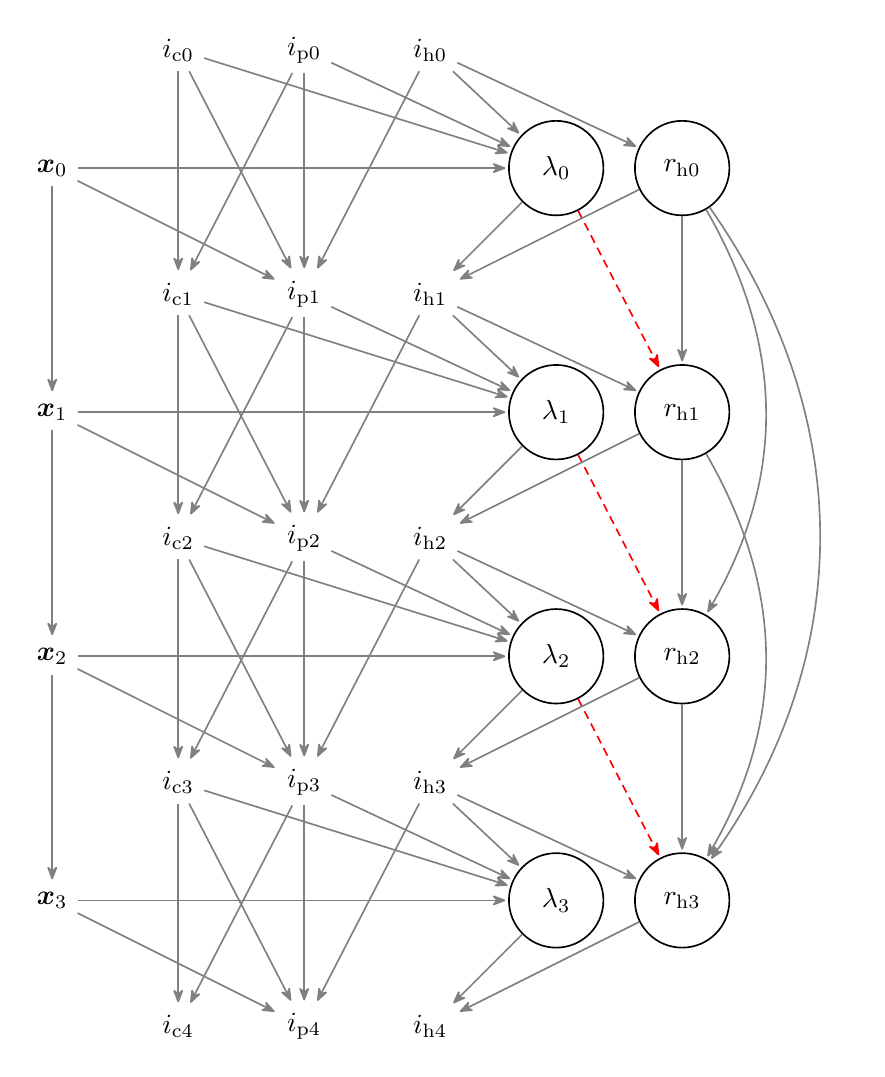
\begin{tikzpicture}[
	>= {Stealth[round]},semithick,black!50,
	text=black, 
	node distance = 1.6cm, 
	every new ->/.style={shorten >=1pt},
	graphs/every graph/.style={edges=rounded corners}
	]
	
	%% time 0
	\node (empty01) { };
	\node (ic0) [right of=empty01]  {$i_{\mathrm{c}0}$};		
	\node (ip0) [right of=ic0] {$i_{\mathrm{p}0}$};
	\node (ih0) [right of=ip0] {$i_{\mathrm{h}0}$};
	\node (empty05) [right of=ih0] { };
	\node (empty06) [right of=empty05] { };
	\node (x0) [below of=empty01,yshift=1mm] {$\bm{x}_0$};
	\node (empty02) [right of=x0] { };
	\node (empty03) [right of=empty02] { };
	\node (empty04) [right of=empty03] { };
	\node (l0)[unobserved] [right of=empty04] {$\lambda_0$};
	\node (r0)[unobserved] [right of=l0] {$r_{\mathrm{h}0}$};
	
	%% time 1
	\node (empty11) [below of=x0] { };
	\node (ic1) [right of=empty11]  {$i_{\mathrm{c}1}$};		
	\node (ip1) [right of=ic1] {$i_{\mathrm{p}1}$};
	\node (ih1) [right of=ip1] {$i_{\mathrm{h}1}$};
	\node (empty15) [right of=ih1] { };
	\node (empty16) [right of=empty15] { };
	\node (x1) [below of=empty11,yshift=1mm] {$\bm{x}_1$};
	\node (empty12) [right of=x1] { };
	\node (empty13) [right of=empty12] { };
	\node (empty14) [right of=empty13] { };
	\node (l1)[unobserved] [right of=empty14] {$\lambda_1$};
	\node (r1)[unobserved] [right of=l1] {$r_{\mathrm{h}1}$};

	%% time 2
	\node (empty21) [below of=x1] { };
	\node (ic2) [right of=empty21]  {$i_{\mathrm{c}2}$};		
	\node (ip2) [right of=ic2] {$i_{\mathrm{p}2}$};
	\node (ih2) [right of=ip2] {$i_{\mathrm{h}2}$};
	\node (empty25) [right of=ih2] { };
	\node (empty26) [right of=empty25] { };
	\node (x2) [below of=empty21,yshift=1mm] {$\bm{x}_2$};
	\node (empty22) [right of=x2] { };
	\node (empty23) [right of=empty22] { };
	\node (empty24) [right of=empty23] { };
	\node (l2)[unobserved] [right of=empty24] {$\lambda_2$};
	\node (r2)[unobserved] [right of=l2] {$r_{\mathrm{h}2}$};
	
	%% time 3
	\node (empty31) [below of=x2] { };
	\node (ic3) [right of=empty31]  {$i_{\mathrm{c}3}$};		
	\node (ip3) [right of=ic3] {$i_{\mathrm{p}3}$};
	\node (ih3) [right of=ip3] {$i_{\mathrm{h}3}$};
	\node (empty35) [right of=ih3] { };
	\node (empty36) [right of=empty35] { };
	\node (x3) [below of=empty31,yshift=1mm] {$\bm{x}_3$};
	\node (empty32) [right of=x3] { };
	\node (empty33) [right of=empty32] { };
	\node (empty34) [right of=empty33] { };
	\node (l3)[unobserved] [right of=empty34] {$\lambda_3$};
	\node (r3)[unobserved] [right of=l3] {$r_{\mathrm{h}3}$};
	
	%% time 4
	\node (empty41) [below of=x3] { };
	\node (ic4) [right of=empty41]  {$i_{\mathrm{c}4}$};		
	\node (ip4) [right of=ic4] {$i_{\mathrm{p}4}$};
	\node (ih4) [right of=ip4] {$i_{\mathrm{h}4}$};
	\node (empty45) [right of=ih4] { };
	\node (empty46) [right of=empty45] { };
	
	%% from time=0 nodes
	\draw[->,shorten >=1pt] (ic0) to (ic1);
	\draw[->,shorten >=1pt] (ic0) to (ip1);
	\draw[->,shorten >=1pt] (ic0) to (l0);
	\draw[->,shorten >=1pt] (ip0) to (ic1);	
	\draw[->,shorten >=1pt] (ip0) to (ip1);
	\draw[->,shorten >=1pt] (ip0) to (l0);
	\draw[->,shorten >=1pt] (ih0) to (ip1);
	\draw[->,shorten >=1pt] (ih0) to (l0);
	\draw[->,shorten >=1pt] (ih0) to (r0);
	\draw[->,shorten >=1pt] (x0) to (x1);
	\draw[->,shorten >=1pt] (x0) to (ip1);
	\draw[->,shorten >=1pt] (x0) to (l0);
	\draw[->,shorten >=1pt] (l0) to (ih1);
	\draw[->,shorten >=1pt,red,densely dashed] (l0) to (r1);
	\draw[->,shorten >=1pt] (r0) to (ih1);
	\draw[->,shorten >=1pt] (r0) to (r1);
	
	%% from time=1 nodes
	\draw[->,shorten >=1pt] (ic1) to (ic2);
	\draw[->,shorten >=1pt] (ic1) to (ip2);
	\draw[->,shorten >=1pt] (ic1) to (l1);
	\draw[->,shorten >=1pt] (ip1) to (ic2);	
	\draw[->,shorten >=1pt] (ip1) to (ip2);
	\draw[->,shorten >=1pt] (ip1) to (l1);
	\draw[->,shorten >=1pt] (ih1) to (ip2);
	\draw[->,shorten >=1pt] (ih1) to (l1);
	\draw[->,shorten >=1pt] (ih1) to (r1);
	\draw[->,shorten >=1pt] (x1) to (x2);
	\draw[->,shorten >=1pt] (x1) to (ip2);
	\draw[->,shorten >=1pt] (x1) to (l1);
	\draw[->,shorten >=1pt] (l1) to (ih2);
	\draw[->,shorten >=1pt,red,densely dashed] (l1) to (r2);
	\draw[->,shorten >=1pt] (r1) to (ih2);
	\draw[->,shorten >=1pt] (r1) to (r2);
	
	%% from time=2 nodes
	\draw[->,shorten >=1pt] (ic2) to (ic3);
	\draw[->,shorten >=1pt] (ic2) to (ip3);
	\draw[->,shorten >=1pt] (ic2) to (l2);
	\draw[->,shorten >=1pt] (ip2) to (ic3);	
	\draw[->,shorten >=1pt] (ip2) to (ip3);
	\draw[->,shorten >=1pt] (ip2) to (l2);
	\draw[->,shorten >=1pt] (ih2) to (ip3);
	\draw[->,shorten >=1pt] (ih2) to (l2);
	\draw[->,shorten >=1pt] (ih2) to (r2);
	\draw[->,shorten >=1pt] (x2) to (x3);
	\draw[->,shorten >=1pt] (x2) to (ip3);
	\draw[->,shorten >=1pt] (x2) to (l2);
	\draw[->,shorten >=1pt] (l2) to (ih3);
	\draw[->,shorten >=1pt,red,densely dashed] (l2) to (r3);
	\draw[->,shorten >=1pt] (r2) to (ih3);
	\draw[->,shorten >=1pt] (r2) to (r3);
	
	%% from time=3 nodes
	\draw[->,shorten >=1pt] (ic3) to (ic4);
	\draw[->,shorten >=1pt] (ic3) to (ip4);
	\draw[->,shorten >=1pt] (ic3) to (l3);
	\draw[->,shorten >=1pt] (ip3) to (ic4);	
	\draw[->,shorten >=1pt] (ip3) to (ip4);
	\draw[->,shorten >=1pt] (ip3) to (l3);
	\draw[->,shorten >=1pt] (ih3) to (ip4);
	\draw[->,shorten >=1pt] (ih3) to (l3);
	\draw[->,shorten >=1pt] (ih3) to (r3);
	\draw[->,shorten >=1pt] (x3) to (ip4);
	\draw[->,shorten >=1pt] (x3) to (l3);
	\draw[->,shorten >=1pt] (l3) to (ih4);
	\draw[->,shorten >=1pt] (r3) to (ih4);
	
	%% longer effects of immunity 
	\draw[->,shorten >=1pt,bend left=30] (r0) to (r2);
	\draw[->,shorten >=1pt,bend left=30] (r1) to (r3);
	\draw[->,shorten >=1pt,bend left=35] (r0) to (r3);
	
\end{tikzpicture}

\end{document}
